\documentclass[lettersize,journal]{IEEEtran}

\usepackage{amsmath,amsfonts}
\usepackage{algorithmic}
\usepackage{algorithm}
\usepackage{array}
\usepackage[caption=false,font=normalsize,labelfont=sf,textfont=sf]{subfig}
\usepackage{textcomp}
\usepackage{stfloats}
\usepackage{url}
\usepackage{graphicx}
\usepackage{cite}

\hyphenation{op-tical net-works semi-conduc-tor L-SHADE}

\begin{document}

\title{Coverage-State-Aware L-SHADE for Dynamic Routing Planning in Heterogeneous UAV Communication Networks}

\author{Author Name%
\thanks{Manuscript prepared from an undergraduate thesis on heterogeneous UAV communication-network routing planning.}
\thanks{Author affiliation and contact information should be completed before submission.}}

\markboth{IEEE Computer Society Journal Draft, June~2026}%
{Author: Coverage-State-Aware L-SHADE for Dynamic UAV Routing Planning}

\maketitle

\begin{abstract}
Heterogeneous unmanned aerial vehicle (UAV) communication networks can rapidly provide coverage, relay forwarding, and data aggregation when terrestrial infrastructure is unavailable or damaged. In such networks, UAVs differ in speed, coverage radius, bandwidth, transmit power, buffer capacity, and energy budget, making dynamic routing planning a coupled control problem rather than a static next-hop selection problem. This paper formulates dynamic routing planning for heterogeneous UAV clusters as a continuous optimization task over UAV speed, heading angle, and transmit power. The model jointly considers UAV mobility, air-to-ground coverage, UAV-to-UAV and UAV-to-sink link rates, queue evolution, energy consumption, coverage violation, and connectivity violation. To solve the resulting high-dimensional, nonlinear, non-smooth, and time-coupled problem, a coverage-state-aware L-SHADE algorithm is proposed. The algorithm introduces coverage-oriented individuals during initialization and uses a coverage-state machine to guide parameter control during the iterative search process. Simulation results show that, compared with the original L-SHADE, the proposed method improves the average coverage rate by about 8.09\%, reduces the normalized coverage violation by about 37.64\%, increases throughput by about 64.25\%, and reduces queue load by about 19.64\%. These results indicate that explicitly incorporating coverage state into evolutionary search is beneficial for dynamic UAV routing planning in emergency communication scenarios.
\end{abstract}

\begin{IEEEkeywords}
Heterogeneous UAV swarm, dynamic routing planning, emergency communication, coverage state awareness, L-SHADE, evolutionary optimization.
\end{IEEEkeywords}

\section{Introduction}
\IEEEPARstart{U}{nmanned} aerial vehicle (UAV) communication networks are attractive for emergency communication, temporary coverage, and regional monitoring because UAVs can be deployed rapidly and can adapt their positions according to the task environment. When ground infrastructure is damaged after a disaster, a UAV cluster may be required to cover ground task nodes, relay generated data, and forward information to a sink node. Compared with static terrestrial networks, such networks are more flexible but also more difficult to optimize because mobility, wireless link quality, queue discharge, and energy consumption evolve together.

The difficulty becomes more pronounced in heterogeneous UAV clusters. Different UAVs may have different speed limits, coverage radii, bandwidths, transmit-power ranges, buffer capacities, and energy budgets. As a result, dynamic routing planning should not be treated only as a fixed-path or next-hop decision. Instead, the control sequence of each UAV---including speed, heading angle, and transmit power---directly affects coverage, link rate, traffic backlog, and energy consumption. The planning problem is therefore high-dimensional, nonlinear, non-smooth, and strongly time-coupled.

Evolutionary computation is a natural candidate for this type of problem because it can handle complex black-box objectives and constraints. In particular, L-SHADE, a differential-evolution variant with success-history adaptation and linear population-size reduction, has shown strong performance on continuous optimization problems. However, directly applying the original L-SHADE to heterogeneous UAV routing planning has two limitations. First, random initialization does not fully exploit the spatial distribution of ground task nodes, which may produce weak initial coverage. Second, parameter adaptation is driven mainly by objective-function improvement and lacks explicit awareness of whether the current population is constructing, maintaining, or losing coverage.

This paper makes the following contributions:
\begin{itemize}
  \item A dynamic routing-planning model is formulated for heterogeneous UAV communication networks by jointly considering mobility, coverage, wireless transmission, queue evolution, energy consumption, and connectivity.
  \item A coverage-state-aware L-SHADE algorithm is developed by combining coverage-oriented initialization with a state-driven parameter-control mechanism.
  \item A simulation study compares the proposed method with the original L-SHADE and analyzes convergence, coverage, throughput, queue load, and energy consumption.
\end{itemize}

\section{Related Work}
UAV communication and routing have been widely investigated in recent years. Surveys on UAV-assisted wireless communication summarize the role of UAVs in 6G-and-beyond networks and highlight trajectory design, resource allocation, channel modeling, and regulatory constraints as central issues \cite{Mahbub2025UAV}. UAV path-planning surveys further show that metaheuristic and learning-based methods are frequently used when the search space is nonlinear, constrained, or difficult to model analytically \cite{Jiang2024Evolutionary,Ghambari2024UAV,Agrawal2024Metaheuristic,Elnabty2022Survey}.

For UAV network routing, recent studies have considered dynamic link states, routing holes, frequency allocation, and joint trajectory control. Reinforcement-learning-based geographic routing can exploit predicted link-state evolution for highly dynamic UAV networks \cite{Xu2026EvoQGeo}, while multi-agent deep reinforcement learning has been used for joint trajectory, frequency, and routing control in UAV swarm networks \cite{Alam2024JointTrajectory}. Bio-inspired routing methods have also been reviewed for flying ad hoc networks, indicating that population-based search remains useful when exact models are difficult to solve \cite{Beegum2023FANETReview}.

Trajectory and coverage optimization are closely related to communication performance. Energy-efficient UAV communication with trajectory optimization demonstrates the strong coupling between movement and transmission energy \cite{Zeng2017EnergyEfficient}, and joint trajectory-and-coverage optimization has been studied for UAV-assisted cellular communication \cite{Li2021CoverageOptimization}. These studies motivate a unified formulation in which coverage, link rate, queue load, and energy are optimized together.

L-SHADE improves SHADE by using linear population-size reduction and success-history-based parameter adaptation \cite{Tanabe2014LSHADE}. It has also been adapted to UAV swarm resource configuration problems \cite{Li2022ALSHADE}. Nevertheless, when the objective includes explicit coverage constraints, the search process can benefit from task-specific state information. This paper therefore augments L-SHADE with coverage-oriented initialization and coverage-state-aware parameter control.

\section{System Model and Problem Formulation}
\subsection{Network Scenario}
Consider a fixed-height two-dimensional emergency communication scenario. The network contains a set of heterogeneous UAVs $\mathcal{U}=\{1,\ldots,N\}$, a set of ground task nodes $\mathcal{K}=\{1,\ldots,K\}$, and one fixed sink node $s$. Time is divided into slots $\mathcal{T}=\{0,\ldots,T-1\}$ and grouped into control segments $\mathcal{G}=\{0,\ldots,G-1\}$. In each segment, every UAV selects speed, heading angle, and transmit power. The decision vector can be written as
\begin{equation}
\mathbf{x}=\{v_{i,g},\theta_{i,g},p_{i,g}\mid i\in\mathcal{U}, g\in\mathcal{G}\},
\label{eq:decision-vector}
\end{equation}
where $v_{i,g}$, $\theta_{i,g}$, and $p_{i,g}$ are bounded by UAV-specific physical limits.

The horizontal position of UAV $i$ at time slot $t$ is denoted by $\mathbf{q}_i(t)=[x_i(t),y_i(t)]^T$. Within a control segment, position is updated according to
\begin{equation}
\mathbf{q}_i(t+1)=\mathbf{q}_i(t)+\Delta t\,v_{i,g}
\begin{bmatrix}
\cos\theta_{i,g}\\
\sin\theta_{i,g}
\end{bmatrix},
\label{eq:motion}
\end{equation}
where $g$ is the segment containing time slot $t$.

\subsection{Coverage and Wireless Transmission}
Ground node $k$ is covered by UAV $i$ at slot $t$ when the horizontal distance is within the UAV's coverage radius:
\begin{equation}
c_{i,k}(t)=
\begin{cases}
1, & \|\mathbf{q}_i(t)-\mathbf{w}_k\|_2 \le R_i,\\
0, & \text{otherwise},
\end{cases}
\label{eq:coverage}
\end{equation}
where $\mathbf{w}_k$ is the position of ground node $k$ and $R_i$ is the coverage radius of UAV $i$. The overall coverage ratio is
\begin{equation}
\rho(t)=\frac{1}{K}\sum_{k=1}^{K}\mathbb{I}\left(\sum_{i=1}^{N}c_{i,k}(t)\ge 1\right).
\label{eq:coverage-ratio}
\end{equation}

For a communication link from node $a$ to node $b$, the achievable rate is modeled by the Shannon expression
\begin{equation}
r_{a,b}(t)=B_{a,b}\log_2\left(1+\frac{p_a(t)h_{a,b}(t)}{\sigma^2}\right),
\label{eq:link-rate}
\end{equation}
where $B_{a,b}$ is the allocated bandwidth, $p_a(t)$ is the transmit power, $h_{a,b}(t)$ is the channel gain, and $\sigma^2$ is the noise power.

\subsection{Queue Evolution and Energy Consumption}
Let $Q_i(t)$ be the data queue of UAV $i$. The queue evolves according to the amount of data collected from covered ground nodes, received from other UAVs, and forwarded to neighboring UAVs or the sink:
\begin{equation}
Q_i(t+1)=\left[Q_i(t)+A_i(t)+I_i(t)-O_i(t)\right]^+,
\label{eq:queue-update}
\end{equation}
where $A_i(t)$ is the collected ground-node traffic, $I_i(t)$ is the incoming relay traffic, $O_i(t)$ is the outgoing traffic, and $[z]^+=\max(z,0)$.

The energy consumption of UAV $i$ includes propulsion and communication components:
\begin{equation}
E_i=\sum_{t=0}^{T-1}\left(P_i^{\mathrm{fly}}(v_i(t))+p_i(t)\right)\Delta t,
\label{eq:energy}
\end{equation}
where $P_i^{\mathrm{fly}}(\cdot)$ denotes the propulsion-power model.

\subsection{Optimization Objective}
The goal is to maximize data delivery and coverage while reducing queue backlog, energy consumption, coverage violation, and connectivity violation. A scalar objective is formed as
\begin{align}
\min_{\mathbf{x}} \quad
F(\mathbf{x})={}&
w_Q\bar{Q}(\mathbf{x})
+w_E\bar{E}(\mathbf{x})
+w_C V_C(\mathbf{x}) \nonumber\\
&+w_L V_L(\mathbf{x})
-w_D\bar{D}(\mathbf{x}),
\label{eq:objective}
\end{align}
subject to mobility, power, queue, energy, coverage, and connectivity constraints. Here $\bar{Q}$ is normalized queue load, $\bar{E}$ is normalized energy consumption, $V_C$ is coverage violation, $V_L$ is connectivity violation, $\bar{D}$ is normalized delivered throughput, and $w_Q,w_E,w_C,w_L,w_D$ are nonnegative weights.

\section{Coverage-State-Aware L-SHADE Algorithm}
\subsection{Motivation}
Original L-SHADE relies on random initialization and adaptive control parameters. Although this mechanism is general, it does not explicitly consider whether the UAV population currently provides adequate coverage. For dynamic routing planning, poor early coverage can lead to weak link construction and queue accumulation, while excessive differential perturbation in later iterations can destroy useful coverage structures. The proposed method introduces coverage information into both initialization and parameter control.

\subsection{Coverage-Oriented Initialization}
The initial population consists of random individuals and coverage-oriented individuals. For coverage-oriented individuals, UAV headings and speeds are biased toward uncovered or weakly covered task-node regions. Transmit powers are initialized within feasible ranges while considering the need to maintain UAV-to-UAV or UAV-to-sink connectivity. This mechanism increases the probability that early candidate solutions contain meaningful coverage structures without eliminating population diversity.

\subsection{Coverage-State Machine}
During evolution, the population is evaluated not only by objective value but also by coverage state. Let $\rho_{\mathrm{best}}$ be the coverage ratio of the best individual, $\rho_{\mathrm{avg}}$ be the population-average coverage ratio, and $\Delta\rho$ be the recent coverage improvement. The coverage state is classified into three modes:
\begin{itemize}
  \item \emph{Construction}: coverage is insufficient and needs aggressive exploration toward task-node regions.
  \item \emph{Maintenance}: coverage is acceptable but fragile, requiring balanced exploration and exploitation.
  \item \emph{Optimization}: coverage is stable, allowing stronger exploitation of throughput, queue, and energy objectives.
\end{itemize}
Fig.~\ref{fig:state-machine} illustrates the state-transition logic.

\begin{figure}[!t]
\centering
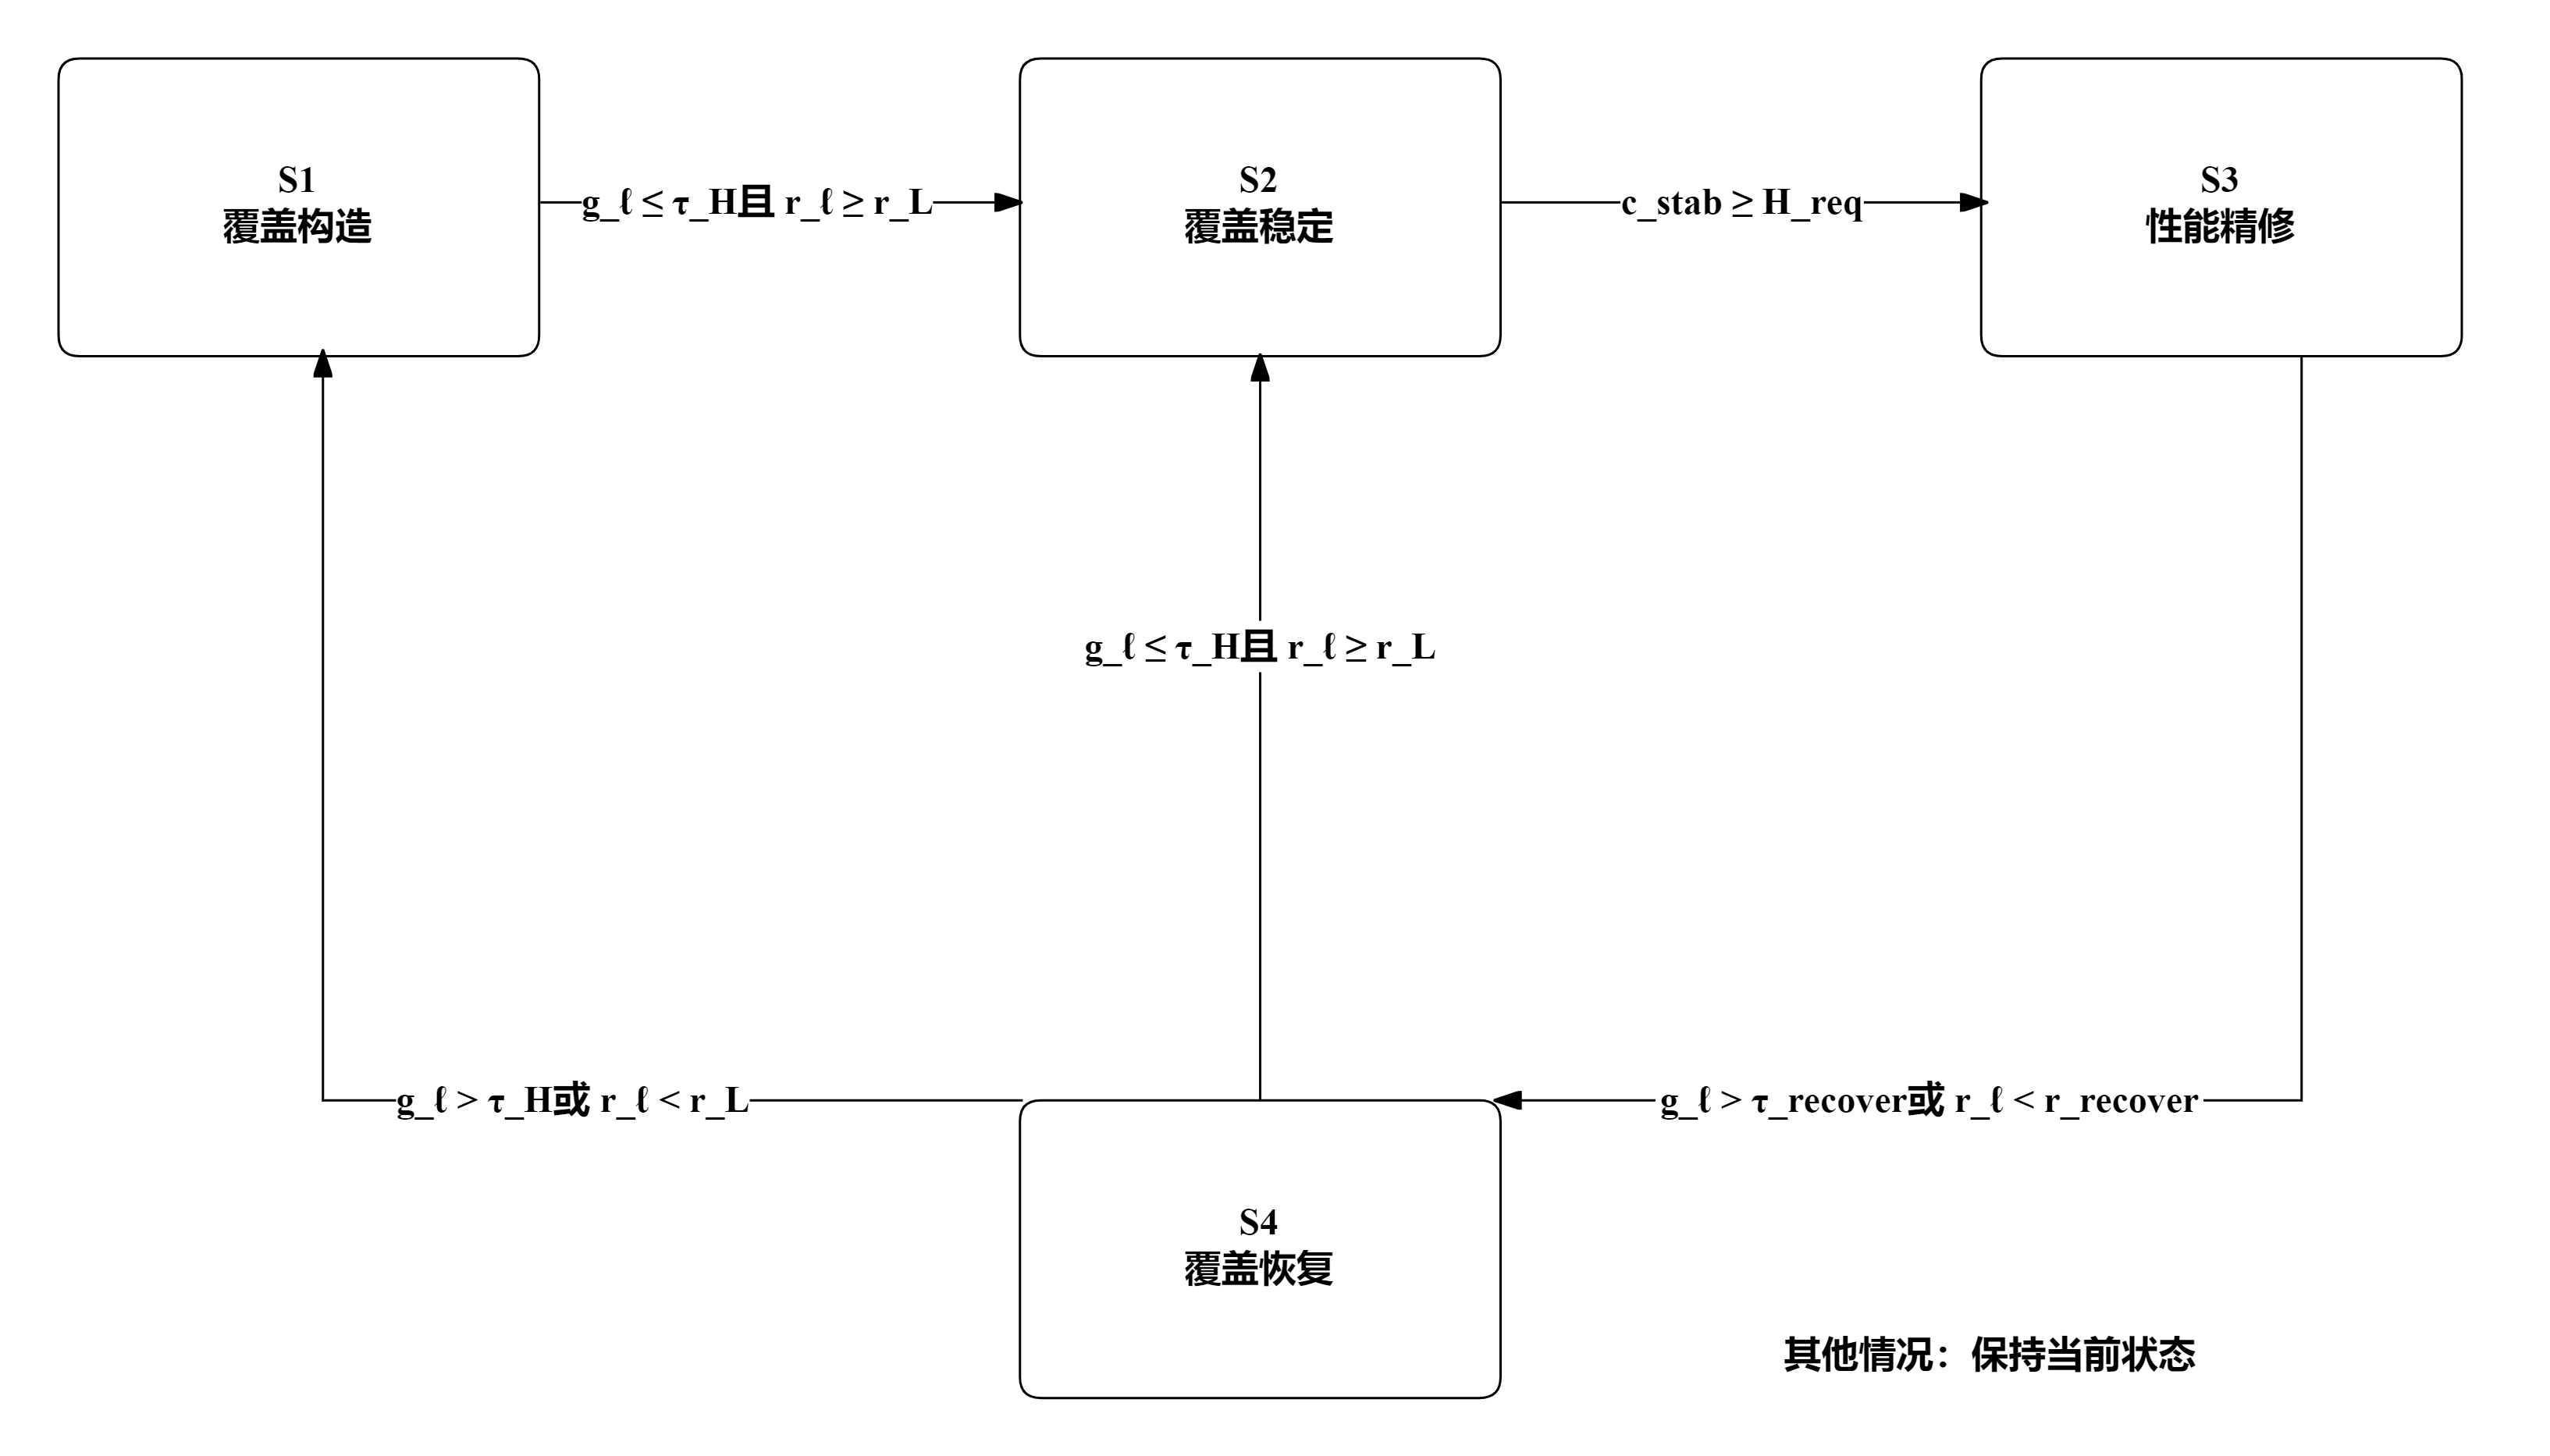
\includegraphics[width=3.2in]{fig_coverage_state_machine}
\caption{Coverage-state machine used to guide L-SHADE parameter control.}
\label{fig:state-machine}
\end{figure}

\subsection{State-Driven Parameter Control}
L-SHADE generates mutation and crossover parameters $F$ and $CR$ from historical memories. The proposed method adjusts the sampling tendency according to the coverage state. In the construction state, larger perturbations and a broader $p$-best range are preferred to improve exploration. In the maintenance state, moderate perturbations are used to preserve existing coverage structures. In the optimization state, smaller perturbations and a more exploitative $p$-best selection are preferred to refine throughput, queue load, and energy consumption.

\begin{algorithm}[!t]
\caption{Coverage-State-Aware L-SHADE}
\label{alg:csa-lshade}
\begin{algorithmic}[1]
\STATE Initialize population with random and coverage-oriented individuals
\STATE Evaluate objective value and coverage indicators
\WHILE{termination criterion is not met}
  \STATE Determine coverage state from population coverage statistics
  \FOR{each target individual}
    \STATE Sample $F$, $CR$, and $p$ according to the current state
    \STATE Generate a mutant vector using current-to-$p$best mutation
    \STATE Apply crossover and boundary repair
    \STATE Evaluate the trial individual
    \STATE Select between target and trial individuals
  \ENDFOR
  \STATE Update parameter memories using successful trials
  \STATE Reduce population size linearly as in L-SHADE
\ENDWHILE
\STATE \textbf{return} the best UAV control sequence
\end{algorithmic}
\end{algorithm}

The computational complexity is dominated by population evaluation. If the population size is $P$, the number of iterations is $I$, the number of UAVs is $N$, the number of task nodes is $K$, and the number of time slots is $T$, the main evaluation cost is approximately $O(IPT(NK+N^2))$, where $NK$ corresponds to coverage evaluation and $N^2$ corresponds to inter-UAV link evaluation.

\section{Simulation Results and Discussion}
\subsection{Experimental Setting}
The simulation considers a fixed heterogeneous emergency communication scenario with multiple UAVs, several ground task nodes, and one sink node. Each candidate solution encodes the UAV speed, heading angle, and transmit power over all control segments. The proposed coverage-state-aware L-SHADE is compared with the original L-SHADE under the same population size, maximum evaluation budget, UAV heterogeneity, and task-node traffic setting. The evaluation metrics include convergence behavior, average coverage ratio, normalized coverage violation, throughput, queue load, and energy consumption.

\subsection{Convergence Performance}
Fig.~\ref{fig:convergence} compares the convergence behavior of the proposed method with the baseline. The coverage-oriented initialization improves the quality of early individuals, while the state-driven parameter-control mechanism reduces unnecessary destruction of useful coverage structures in the middle and later search stages.

\begin{figure}[!t]
\centering
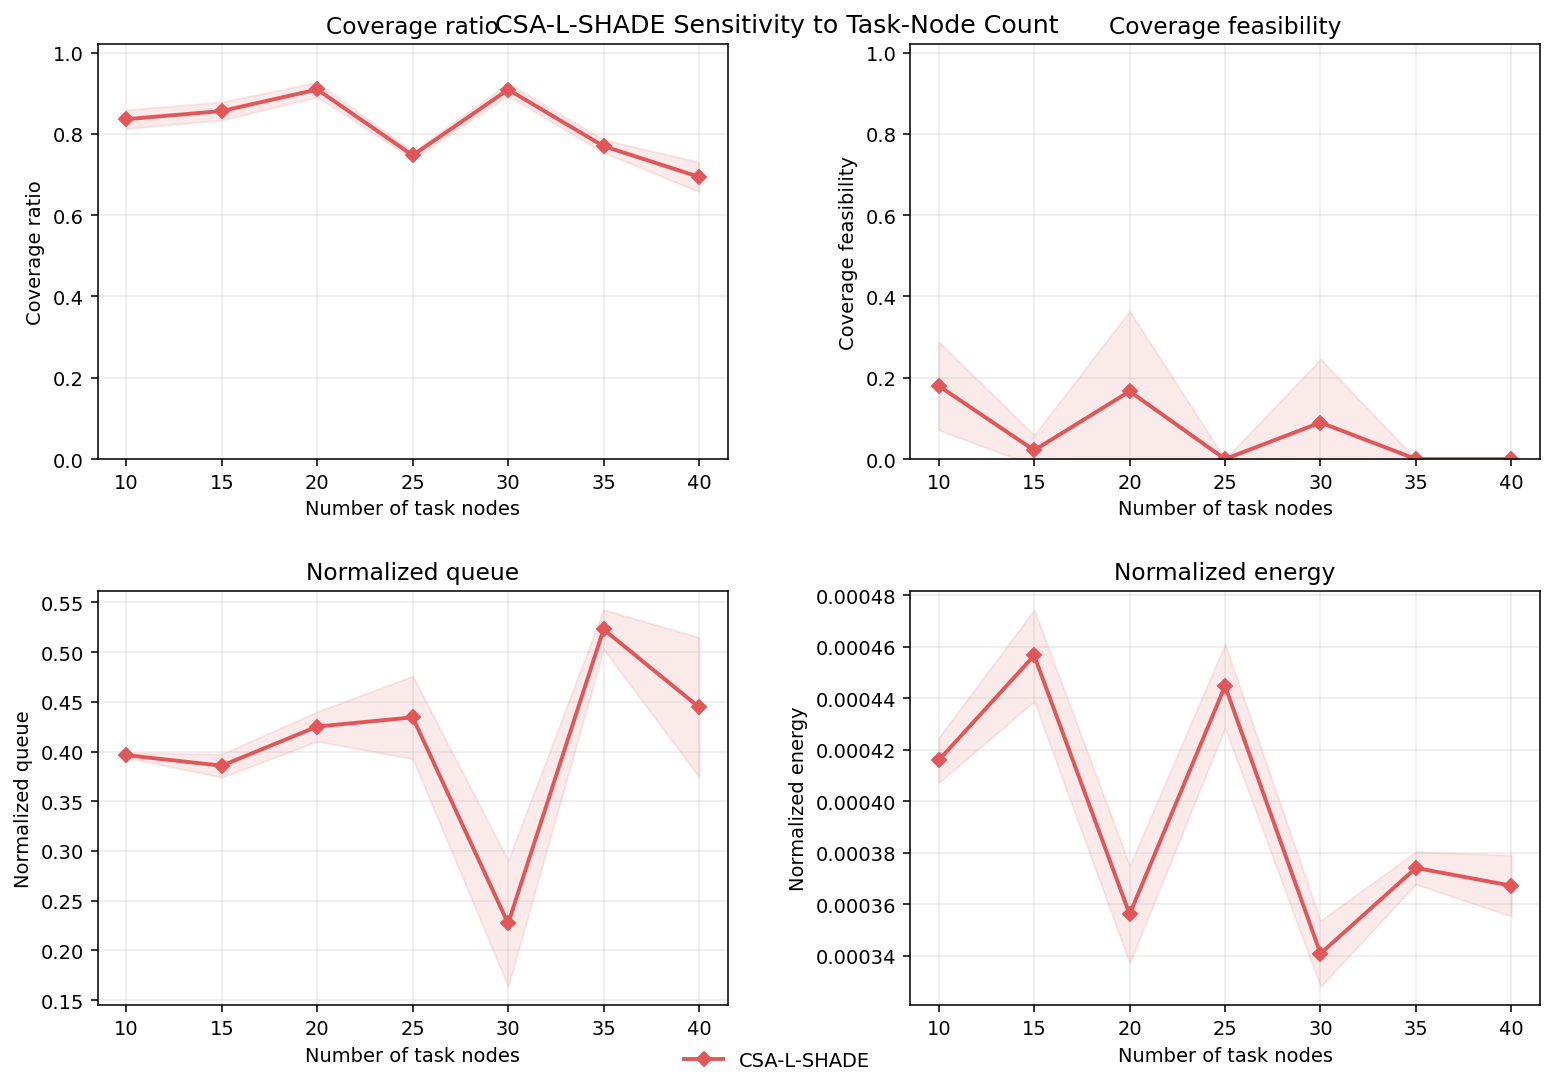
\includegraphics[width=3.4in]{fig_csa_convergence}
\caption{Convergence comparison between the proposed coverage-state-aware L-SHADE and baseline variants.}
\label{fig:convergence}
\end{figure}

\subsection{Coverage Performance}
Coverage is the primary requirement in emergency communication because uncovered task nodes cannot reliably inject data into the aerial network. As shown in Fig.~\ref{fig:coverage-performance}, the proposed method achieves a higher average coverage ratio and lower coverage violation than the original L-SHADE. Quantitatively, it improves the average coverage rate by about 8.09\% and reduces the normalized coverage violation by about 37.64\%. This confirms that using task-node spatial information during initialization and coverage-state information during evolution improves coverage construction and preservation.

\begin{figure}[!t]
\centering
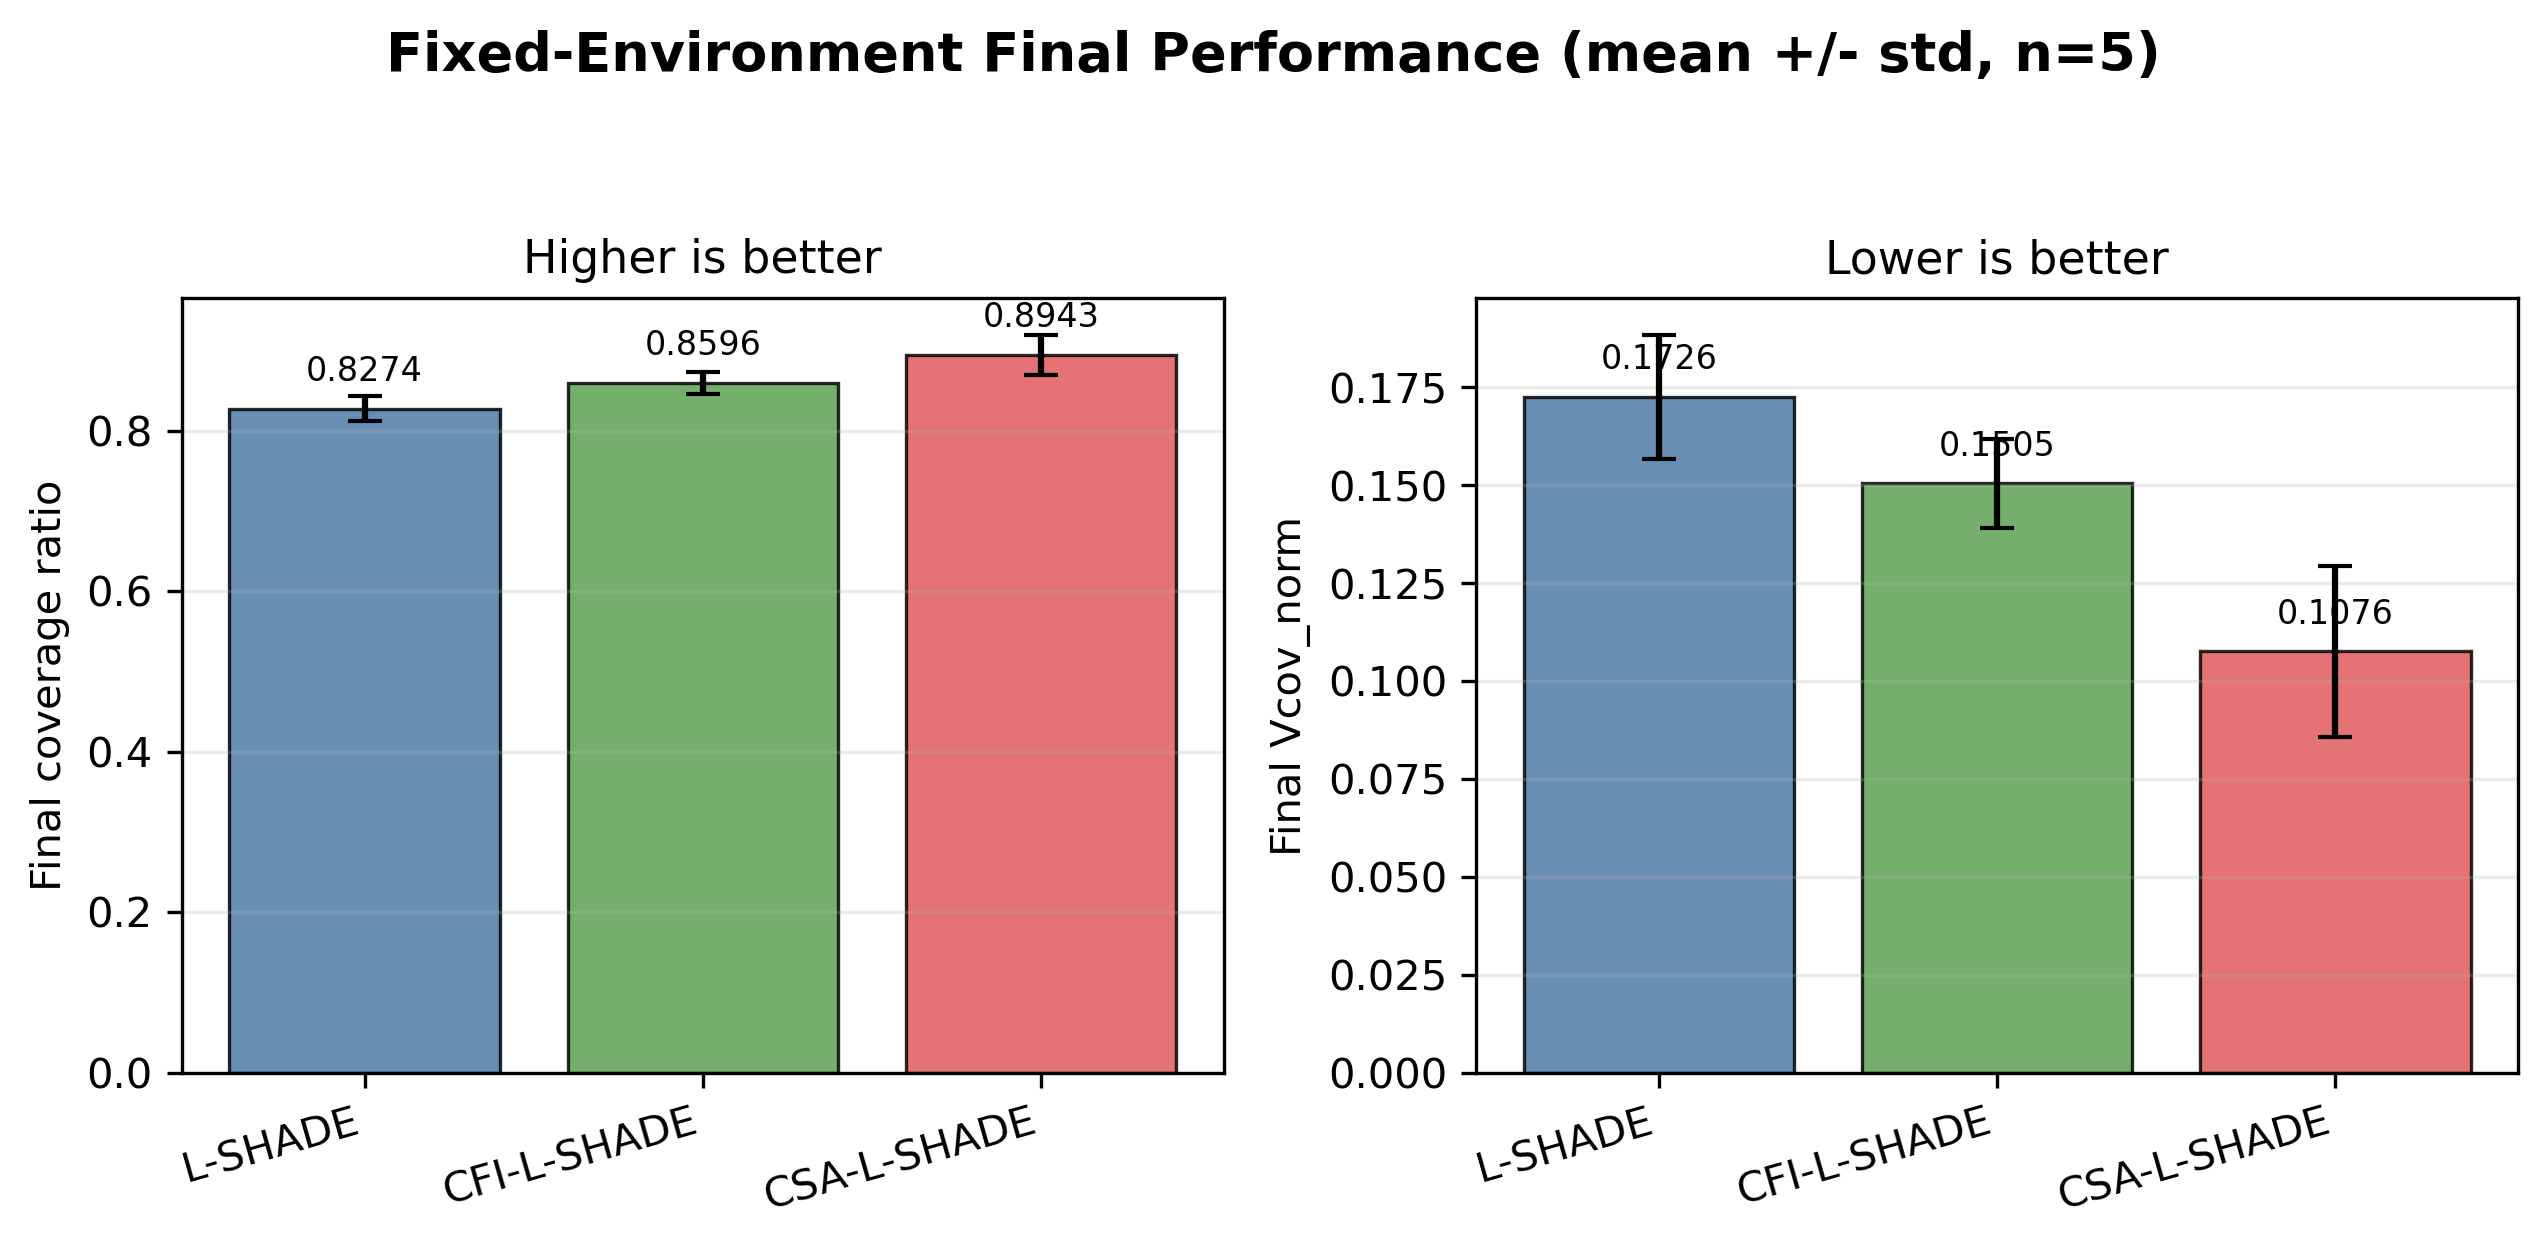
\includegraphics[width=3.4in]{fig_coverage_performance}
\caption{Coverage performance of the proposed method and the baseline.}
\label{fig:coverage-performance}
\end{figure}

\subsection{Communication and Resource Performance}
Figs.~\ref{fig:throughput}--\ref{fig:energy} report throughput, queue load, and energy consumption. Compared with the original L-SHADE, the proposed method increases throughput by about 64.25\% and reduces queue load by about 19.64\%. The improvement is consistent with the modeling logic: better coverage allows more task-node data to enter the UAV network, and more stable link construction helps discharge queues toward the sink. Energy consumption remains controlled because the objective penalizes excessive motion and transmit power.

\begin{figure}[!t]
\centering
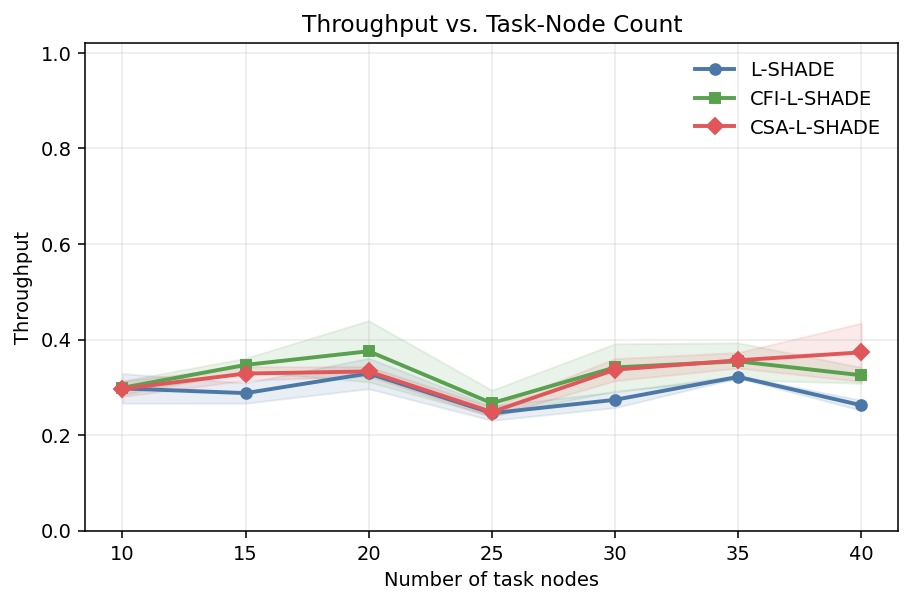
\includegraphics[width=3.4in]{fig_throughput}
\caption{Delivered throughput comparison.}
\label{fig:throughput}
\end{figure}

\begin{figure}[!t]
\centering
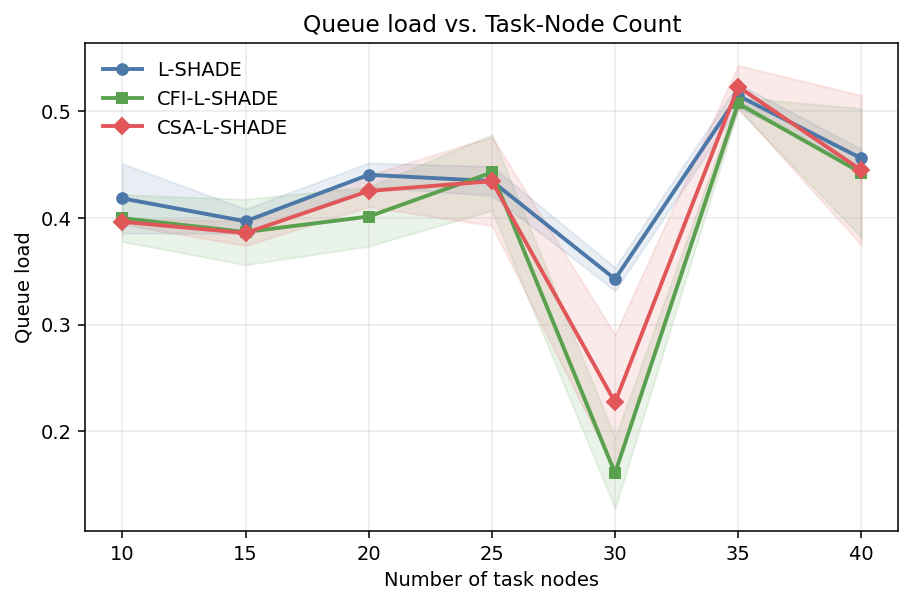
\includegraphics[width=3.4in]{fig_queue_load}
\caption{Queue-load comparison.}
\label{fig:queue-load}
\end{figure}

\begin{figure}[!t]
\centering
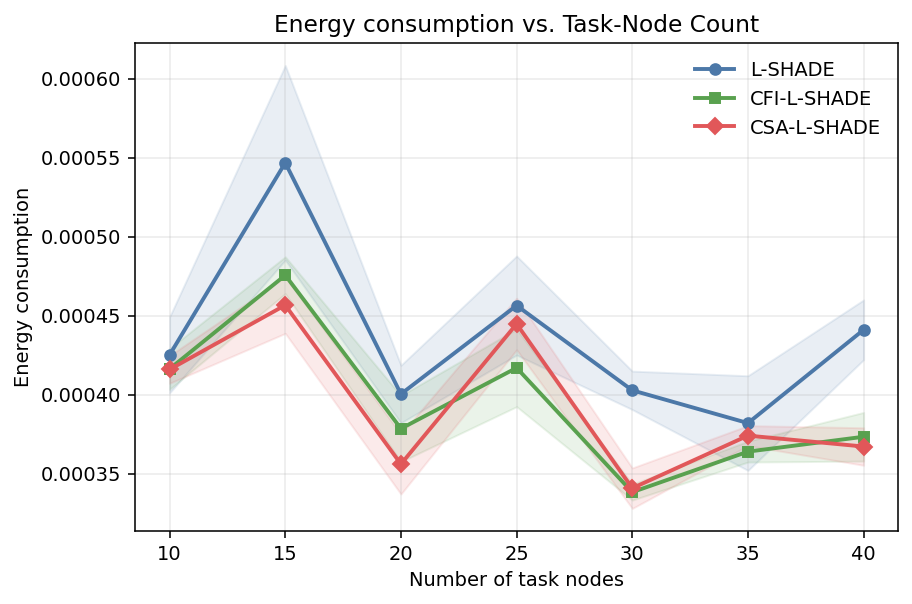
\includegraphics[width=3.4in]{fig_energy_consumption}
\caption{Energy-consumption comparison.}
\label{fig:energy}
\end{figure}

\subsection{Discussion}
The results suggest that coverage state is not merely an evaluation metric but also useful guidance for evolutionary search. Coverage-priority initialization mainly alleviates insufficient initial coverage, whereas state-driven parameter control reduces the chance that differential perturbation destroys already formed coverage structures. The proposed method is therefore suitable for scenarios in which UAVs must rapidly build and maintain a communication backbone under heterogeneous constraints.

The current study is simulation-based and assumes a fixed-height two-dimensional environment. Before strict journal submission, the method should be further evaluated under more channel models, mobility disturbances, larger-scale topologies, and real or semi-realistic traffic traces.

\section{Conclusion}
This paper presented a coverage-state-aware L-SHADE algorithm for dynamic routing planning in heterogeneous UAV communication networks. The routing-planning problem was formulated as a continuous optimization problem over UAV speed, heading angle, and transmit power, with joint consideration of coverage, link rate, queue evolution, energy consumption, and connectivity. The proposed algorithm combines coverage-oriented initialization and coverage-state-driven parameter control to adapt the search process to coverage construction, maintenance, and performance optimization. Simulation results showed clear improvements over original L-SHADE in coverage, throughput, and queue load. Future work will extend the model to more realistic three-dimensional mobility, uncertain channels, and online replanning.

\bibliographystyle{IEEEtran}
\bibliography{references}

\end{document}
